\section{Identification des demandes des parties}
\subsection{Objectif de la tâche}
\begin{frame}[t]{\mysubsectiontitle}
\begin{exampleblock}{\scriptsize Exemple : dommage-intérêts pour procédure abusive (danais)}
	%danais/CASAI1401082.xml
	\scriptsize
	Jennifer M. et Catherine M. ... demandent à la Cour de :
	
	- \textcolor{red}{infirmer le dit jugement} en \textcolor{blue}{toutes ses dispositions} ; 
	...
	
	Statuant à nouveau ...
	
	- les condamner au paiement d' une somme de  \textbf{3 000,00 \euro pour procédure abusive} et
	aux entiers dépens ; ...
	
	La cour ... CONFIRME \textcolor{red}{le jugement entrepris} en \textcolor{blue}{toutes ses dispositions}.
	
	\centering 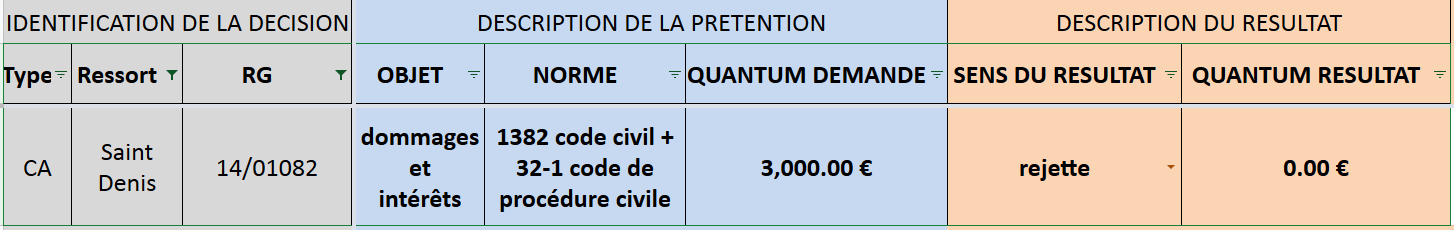
\includegraphics[width=0.8\textwidth]{tab-danais.png}
\end{exampleblock}

\begin{alertblock}{\scriptsize Difficultés}
	\begin{itemize}\scriptsize 
		\item Présence de plusieurs demandes de catégories similaires et/ou différentes dans une même décision
		\item Toutes les catégories ne sont pas connues d'avance (+500 catégories)
		\item Difficile d'annoter une base d'évaluation pour toutes les couvrir
		\item Enoncés non structurés, avec des références, et des agrégations
	\end{itemize}
\end{alertblock}
\end{frame}

\subsection{Méthode proposée}

\begin{frame}[t]{\mysubsectiontitle}
%	\begin{itemize}	\scriptsize
%		\item Phase d'entraînement	
%		\begin{itemize} \scriptsize
%			\item entraînement d'un classifieur pour détecter la présence d'une catégorie
%			\item Détermination automatique de la terminologie de la catégorie : 
%		\end{itemize}
%	\item Phase d'extraction
	\begin{enumerate} \scriptsize
		\item Détermination automatique de la terminologie (déclencheurs) de la catégorie \[ngl(t,c) = \frac{\sqrt{N} (N_{t,c} N_{\overline{t},\overline{c}}) - (N_{t,\overline{c}} N_{\overline{t},c})}{\sqrt{N_t N_{\overline{t}} \vert D_c \vert \vert D_{\overline{c}} \vert }}.\]
		\item Détection de la présence de la catégorie par classification de la décision ($c$ vs. $\overline{c}$)
		\item Identification des passages de demandes et résultats 
		\item Exploiter la proximité entre les déclencheurs de la catégorie  et sommes d’argent pour extraire les quanta:
		
		Section Litige : identification de la demande
		
		\fbox{\parbox{0.8\textwidth}{\scriptsize
				Jennifer M. et Catherine M. ... demandent à la Cour de :
				
				- infirmer le dit jugement en toutes ses dispositions ; 
				...
				
				Statuant à nouveau ...
				
				- \textbf{[} les \underline{condamner} au paiement d' une somme de  \fbox{\parbox{0.13\textwidth}{\textit{\fontfamily{qcs}\selectfont{3 000,00 \euro}}}} \textbf{pour procédure abusive} et
				aux entiers dépens ; \textbf{]}$_\text{demande\_danais}$
				
				 ...							
		}}
	
	Section Dispositif : identification du résultat
	\fbox{\parbox{0.8\textwidth}{\scriptsize			
			La cour ... 
			
			CONFIRME le jugement entrepris en toutes ses dispositions.
	}}
		\item Mise en correspondance des informations relatives à la même demande
	\end{enumerate}
	
%	\end{itemize}
\end{frame}
\subsection{Résultats expérimentaux}
\begin{frame}[t]{\mysubsectiontitle}
	Données
	\begin{figure}[!htb]
		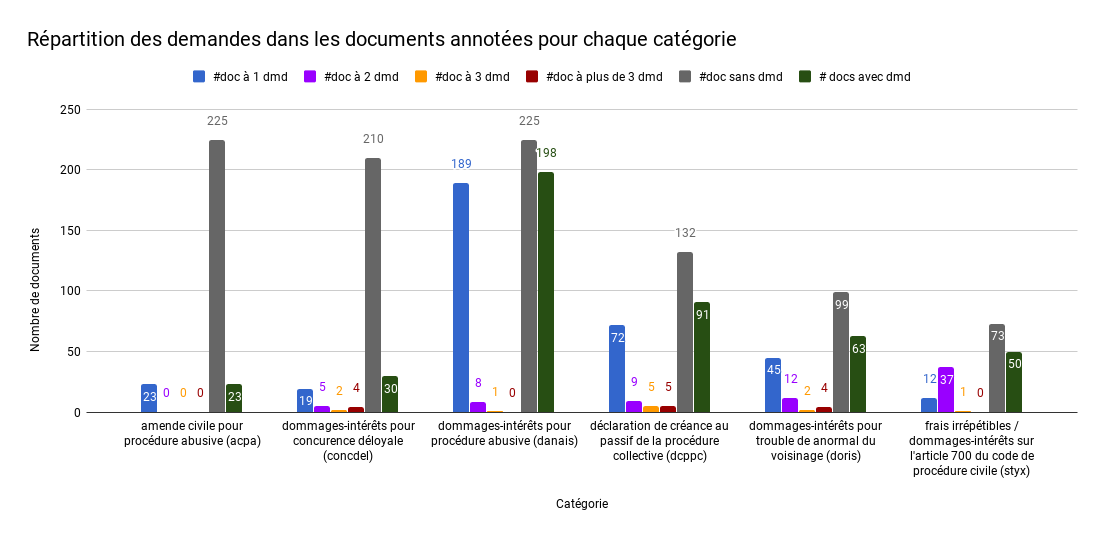
\includegraphics[width=0.8\textwidth]{chartDataset.png}
		\caption{\scriptsize Répartitions des demandes dans les documents annotées.}\label{fig:quanta:hist-repartition-docs}
	\end{figure}	
\end{frame}


\begin{frame}[t]{\mysubsectiontitle}
	Efficacité de la méthode
	\begin{itemize} \scriptsize
		\item Détection de catégorie facile par des classifieurs traditionnels (K-plus-proches-voisins, SVM, Bayésien naïf, Arbre) : $98.8\% \leq$ F$_1$-mesure $\leq 100\%$
		\item Résultat plus facile à extraire que le montant
			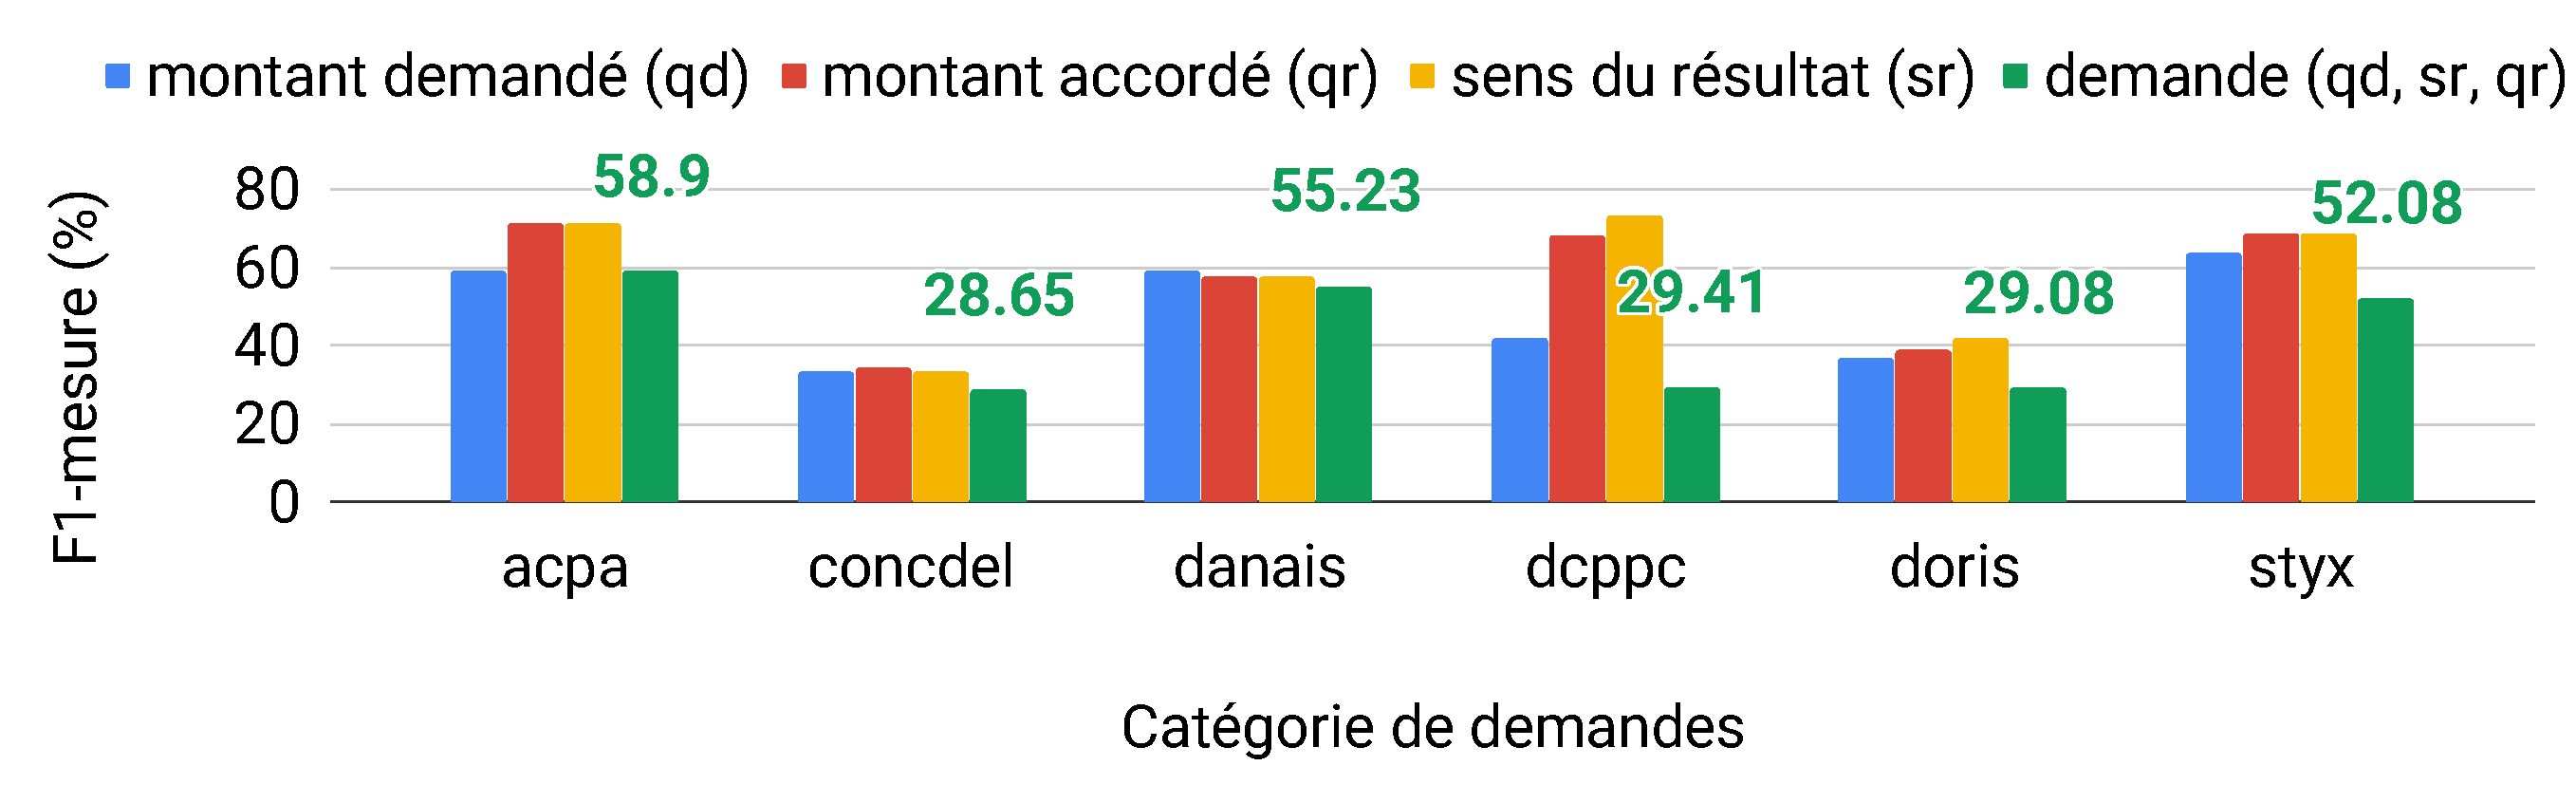
\includegraphics[width=0.8\textwidth]{f1-quanta-et-sens.pdf}			
		\item Source d'erreurs:
		\begin{itemize} \scriptsize
			\item Sélection	difficile de déclencheurs rares
			\item Non exploitation des références aux jugements antérieurs
			\item Certains quanta sont absents des sections Litige et Dispositif
			\item Mauvaise méthode de mise en correspondance
		\end{itemize}
	\end{itemize}
\end{frame}
